\documentclass{beamer}
\DeclareGraphicsExtensions{.pdf,.jpg,.eps}
\definecolor{grisbleu}{rgb}{0.85,0.85,1}
\mode<beamer>{%
  \beamertemplatesolidbackgroundcolor{grisbleu}
 % \usetheme{Paloalto}
  %\usetheme{Montpellier}
  \usetheme{Pittsburgh}
  \usefonttheme{serif,professionalfonts}
}

\mode<trans>{\usetheme{Pittsburgh}}
%%%%%%%%%%%%%%%%%%%%%%%%%%%%%%%%%%%%%%%%%%%%%%%%%%%%%%%%%%%%%%%%%

%\DeclareGraphicsRule{*}{mps}{*}{} % Figures MetaPost

\usepackage{pgf,pgfarrows,pgfnodes}

%\usepackage{pdfcolmk}

% Options pour hyperref.sty
\hypersetup{pdfnewwindow=false}
%\hypersetup{pdfpagemode=FullScreen}
 \setbeamercovered{dynamic}
   \setbeamertemplate{background canvas}[vertical shading][bottom=red!10,top=blue!10]
\usepackage{amsmath}

\usepackage{xmpmulti}
%\usepackage[latin1]{inputenc}
\usepackage[T1]{fontenc}
%\usepackage[oldstyle,upright]{fourier}
\usepackage[upright]{fourier}% Si on n'a pas les compl\'{e}ments expert...
% sf = helvetica scaled 88%
\usepackage[scaled=.88]{helvet}
% tt = lmtt
\renewcommand{\ttdefault}{lmtt}
\newcommand{\Abf}{{\bf A}}
\newcommand{\Bcal}{\mathcal{B}}
\newcommand{\C}{C}
\newcommand{\Esp}{\mathbb{E}}
\newcommand{\eps}{\varepsilon}
\newcommand{\epsbar}{\overline{\eps}}
\newcommand{\etabar}{\overline{\eta}}
\newcommand{\fbf}{{\bf f}}
\newcommand{\Gcal}{\mathcal{G}}
\newcommand{\Hbf}{{\bf H}}
\newcommand{\Ibb}{\mathbb{I}}
\newcommand{\Kcal}{\mathcal{K}}
\newcommand{\lambdabar}{\overline{\lambda}}
\newcommand{\Lcal}{\log \mathcal{L}}
\newcommand{\Mcal}{\mathcal{M}}
\newcommand{\Ncal}{\mathcal{N}}
\newcommand{\Pcal}{\mathcal{P}}
\newcommand{\Qcal}{\mathcal{Q}}
\newcommand{\pibar}{\overline{\pi}}
\newcommand{\pibf}{\mbox{\mathversion{bold}{$\Pi$}}}
\newcommand{\rhobar}{\overline{\rho}}
\newcommand{\Sbf}{{\bf S}}
\newcommand{\Vcal}{\mathcal{V}}
\newcommand{\Vsf}{\mathsf{V}}
\newcommand{\Xcal}{\mathcal{X}}
%\newcommand{\Zbf}{{\bf Z}}
\newcommand{\Zcal}{\mathcal{Z}}
\newcommand{\wbf}{{\bf w}}

%\usepackage[frenchb]{babel}
\mode<beamer>
\makeatletter
\DeclareRobustCommand\sfrac[1]{\@ifnextchar/{\@sfrac{#1}}%
                                          {\@sfrac{#1}/}}
\def\@sfrac#1/#2{\leavevmode\kern.1em\raise.5ex
         \hbox{$\m@th\mbox{\fontsize\sf@size\z@
                           \selectfont#1}$}\kern-.1em
         /\kern-.15em\lower.25ex
          \hbox{$\m@th\mbox{\fontsize\sf@size\z@
                            \selectfont#2}$}}
\makeatother

\newcommand{\Indic}{{\mathbb I}}
% Texte
\usepackage{lscape,fancyhdr, rotating, enumerate,psfig}
%Title "Introduction to networks from a statistical point of view"
%
%Abstract This general presentation gives an overview about
%relevant questions and statistical methods for networks. Many
%scientific communities in the world are working about statistical
%methods for handling complex networks in nature and society, with
%quite different points of view and types of publications. However
%the intersection between them shows common elements which make up
%a new domain of  probability, statistical and computer science.
%The presentation will give some basic notations about networks.
%Then the following questions and methods for handling them will be
%skimmed over: - Detection of  modules or communities from network
%topology, unsupervised classification of vertices. - Prediction of
%the color of a vertex using information about its neighbors. -
%Dynamic models for random graphs such as linear preferential
%attachment - Static models for random graphs: Erdos-Renyi,
%exponential random graphs, latent class models. - Motifs in
%networks. - Sampling questions. - Future: need for models, precise
%and computationally efficient estimates and high quality data.


%%%%%%%%%%%%%%%%%%%%%%%%%%%%%%%%%%%%%%%%%%%%%%%%%%%%%%%%%%%%%%%%%%%%%%
%%%%%%%%%%%%%%%%%%%%%%%%%%%%%%%%%%%%%%%%%%%%%%%%%%%%%%%%%%%%%%%%%%%%%%
\title{Introduction to networks from a statistical point of view}
\author[J.J. Daudin]{Jean-Jacques Daudin,
 UMR $AgroParisTech/INRA518$}

\date{Statistics of Networks,  Royal Statistical Society, \\ 13 November 2007,}
\begin{document}
\begin{frame}
\titlepage
\begin{tabular}{lr}
 \includegraphics[height=1.5cm ] {SSB.png} & \includegraphics[height=1.5cm ] {logagroptech.png} \\
\end{tabular}
\end{frame}

\section{introduction}
\begin{frame}
\frametitle{ISI WEB of Knowledge Essential Science Indicators
Research Fronts rankings in Mathematics, {\small sorted by
Citations}} {\small
\begin{tabular}{|p{1cm}|p{4cm}|p{1cm}|p{1cm}|p{1cm}|p{1cm}|}
  % after \\: \hline or \cline{col1-col2} \cline{col3-col4} ...
  \hline
{\small Rank}   & Research Front &  {\tiny Core Papers} & {\tiny Citations} & {\tiny Citations / paper }& {\tiny Mean year} \\
\hline
  1 & {\small \alert {Complex networks}, Statistical mechanics, Structure, Function, Evolution}  & 3 & 3415 & 1138 & 2002.3 \\
   \hline
  2 & {\small Current-driven magnetic domain wall motion}  & 27 & 1385 & 51.3 & 2004.6
  \\ \hline
  3 & {\small False discovery rate procedure } & 9 & 936 & 104 & 2003.3
  \\ \hline
  4 & {\small Evolutionary game dynamics, \alert {Social networks}}  & 12 & 382 & 31.83 & 2004.8
  \\ \hline
  5 & {\small Porous plate using homotopy analysis method}  & 12 & 359 & 29.92 & 2003.7 \\
  \hline
\end{tabular}
}
\end{frame}

\begin{frame}
\frametitle{ISI WEB of Knowledge Essential Science Indicators
Research Fronts rankings in Mathematics, {\small sorted by Year}}
{\small
\begin{tabular}{|p{1cm}|p{4cm}|p{1cm}|p{1cm}|p{1cm}|p{1cm}|}
  % after \\: \hline or \cline{col1-col2} \cline{col3-col4} ...
  \hline
{\small Rank}   & Research Front &  {\tiny Core Papers} & {\tiny Citations} & {\tiny Citations / paper }& {\tiny Mean year} \\
\hline
  1 & {\small \alert { Exponential random graph (p) models, Curved exponential family models, Social networks }}  & 4 & 16 & 4 & 2006.7 \\
   \hline
  2 & {\small Adaptive/flexible clinical trial design, Confirmatory clinical trials}  & 5 & 17 & 5.6 & 2006 \\
   \hline
  3 & {\small BOSE-EINSTEIN condensation  } & 2 & 9 & 4.5 & 2006
  \\ \hline
  4 & {\small CHEBYSHEV Series form, Computing real roots}  & 3 & 15 & 5 & 2006 \\
  \hline
\end{tabular}
}
\end{frame}

\begin{frame}
\frametitle{Attractive workshops in attractive places}
\includegraphics[height=15cm ] {complexity[1].pdf}
\end{frame}

\begin{frame}

\frametitle{Workshop ERICE 2006}

{\bf Biological systems} show emergent properties that are not
readily explainable by the study of their constituent parts...

 {\bf New mathematical formalisms}, based on
graph theory, are emerging in order to represent and study the
underlying interaction networks present in the cell.

The understanding of the {\bf evolution and organization of these
networks} is changing the way scientists look at biology.

 More specifically, the meeting will focus on:
 \begin{itemize}

 \item gene regulation
 \item metabolic pathways analysis
 \item protein-protein interactions
 \end{itemize}
\end{frame}

\begin{frame}

\frametitle{Complex networks = a speculative bubble or a true new
scientific topic for statisticians ?}
\begin{enumerate}
    \item The network representation of data and questions
    \item Some basic definitions
    \item Characterization of networks using topological motifs
    \item Node clustering
    \item Class prediction for the nodes
    \item Statistical models for networks
    \item Conclusions
\end{enumerate}
\end{frame}

\section{Network representation of data and questions}

\begin{frame}
\frametitle{Network representation of data and questions}
\end{frame}

\begin{frame}
\frametitle{An unusual data set structure}

\begin{tabular}{cc}

  % after \\: \hline or \cline{col1-col2} \cline{col3-col4} ...
  Usual i.i.d. structure & \alert{Structure for relational data} \\

  \begin{tabular}{|c|c|c|c|c|}
    \hline
    % after \\: \hline or \cline{col1-col2} \cline{col3-col4} ...
    item &$X_1$ & ... & ... & $X_p$\\
    \hline
    1 & $x_{11}$ & ... & ... & $x_{1p}$ \\
    2 & $x_{21}$ & ... & ... & $x_{2p}$ \\
    . & . & . & . & . \\
    $n$ & $x_{n1}$ & ... & ... & $x_{np}$ \\
    \hline
  \end{tabular}
     &
     \alert{
\begin{tabular}{|c|c|c|}
    \hline
    item1 & item2 & $R$ \\
    \hline
    1 & 2 & $r_{12}$  \\
    1 & 3 & $r_{13}$ \\
    . & . & .  \\
    $n-1$ & $n$ & $r_{n-1,n}$  \\
    \hline
  \end{tabular}
  }
  \\
\end{tabular}

\begin{itemize}
    \item In the relational data set, the core information is the relation
between two items.
    \item lines are not independent
    \item the data structure is similar to distance, similarity, covariance or
    correlation matrices
    \item \alert{the two types of structures may be combined: information
    about items + information about relations between them.}
\end{itemize}

\end{frame}

\begin{frame}
\frametitle{Representations of a correlation matrix by a graph}
{\small
\begin{tabular}{p{3.5cm} p{3.5cm} p{3.5cm}}
  % after \\: \hline or \cline{col1-col2} \cline{col3-col4} ...
  \vspace{-2.5cm}
 \begin{equation*}
     \left(%
\begin{array}{cccc}
  1 & 0.8 & 0.5 & 0.2 \\
   & 1 & 0.1 & 0.1 \\
   &  & 1 & 0.1 \\
   &  &  & 1 \\
\end{array}%
\right)
\end{equation*} & \includegraphics[height=2.5cm ]
{Graphe-Correlation_value.png} &
 \includegraphics[height=2.5cm ] {Graphe-Correlation_binaire.png} \\

  Correlation matrix& Valued graph & Binary graph using 0.15 threshold \\
  Not readable if more than 10 items & Not readable if more than 10 items & Clusters and hubs appears,
   but the result depends on the threshold used and the representation software. \\
\end{tabular}
Other graphical representations are possible: colored intensity
matrix, PCA... }
\end{frame}

\begin{frame}
\frametitle{Why do people represent data by a network (1) ?}
\begin{tabular}{p{5cm}p{5cm}}
  \vspace{-2cm} \hspace{-5cm}
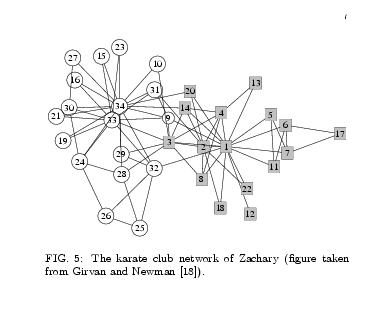
\includegraphics[scale=0.5, angle=-90]{graphe_karate.pdf}\\ &
\vspace{-9cm} \begin{itemize}
    \item Real networks do exist: electric, transport or www
    networks...They have been represented for a long time by
    virtual networks.
    \item Virtual network is a nice way for representing or even "modelling"  many
    scientific phenomenons: social relations, metabolic pathways,
    chemical reactions...
\end{itemize}     \\

\end{tabular}

\end{frame}

\begin{frame}
\frametitle{Why do people represent data by a network (2) ?}
\begin{tabular}{p{7cm}p{3.5cm}}
  \vspace{-0.5cm}
\includegraphics[scale=0.32] {Barabasi6.png} & \begin{itemize}
    \item an overall representation of the interactions between many nodes
    \item the plot reveals the topology of the networks
    \item nodes may be colored, adding more information
\end{itemize}     \\

\end{tabular}

\end{frame}

\begin{frame}
\frametitle{Why do people represent data by a network (3) ?}
\begin{tabular}{p{6cm}p{5cm}}
  \hspace{-1cm}
\includegraphics[scale=0.20] {Framingham_heart_study.png} &
\vspace{-5cm}\begin{itemize}
    \item nodes may be of different sizes, adding more information
    \item edges may be colored, adding more information
    \item a movie may report the evolution of the network in time.
\end{itemize}     \\
\end{tabular}
{\tiny  2200 persons (nodes) from the Framingham Heart study.
Circles with red borders = women, circles with blue borders = men.
The size of each circle is proportional to BMI. The color of the
circles indicates the person's obesity status: yellow = obese
person  and green = nonobese person. The colors of the ties
between the nodes indicate the relationship between them: purple
denotes a friendship or marital tie and orange denotes a familial
tie. N.A. Christakis et al. N Engl J Med, 2007, July}
\end{frame}

\begin{frame}
\frametitle{Choice of the level of detail of the information to be
included in the (metabolic) network} Three possibilities:
\begin{itemize}
    \item (a) include the catalyst Mg2+,
    \item (b) include the co-factors ADP, ATP,...
    \item (c) skeleton information.
\end{itemize}

{\tiny CTP: Cyticline triphosphate, GLC: Aldo-hexose glucose, UDP
: Uticline diphosphate, UMP: Uridine monophosphate, UTP: Uricline
triphosphate, from Barabasi et al} \vspace{0cm} .
\includegraphics[scale=0.4 ] {chaineMetabolique.png}
\end{frame}

\begin{frame}
\frametitle{Tools for visually exploring networks}
\begin{itemize}
    \item No unique representation
    \item Many tools and softwares
    \item See a review for biological networks from M. Suderman and M. Hallet in
    Bioinformatics,vol 23, 2007.
\end{itemize}
\end{frame}

\begin{frame}
\frametitle{Questions induced by the network representation of the
data: the focus is on topological questions(1)}

\begin{tabular}{p{7.5cm}p{5cm}}

\vspace{0cm} \hspace{0cm}{\small  Are there clusters composed of
highly connected nodes?
    something like connected components in a weak sense. \begin{itemize}
        \item This
    question is related to the question of the existence of
    functional modules in biological networks, i.e.  sub-networks
    which can produce outputs independently.
        \item  the second rule of Descartes's method is
        {\it Diviser chacune des difficult�s ... en autant de parcelles
        qu'il se pourrait ... pour les mieux r�soudre. }
        Each cluster may be studied independently and thus
        we are allowed to work on lower sized networks.
    \end{itemize}}
    &
     \vspace{0cm} \hspace{-2.5cm}
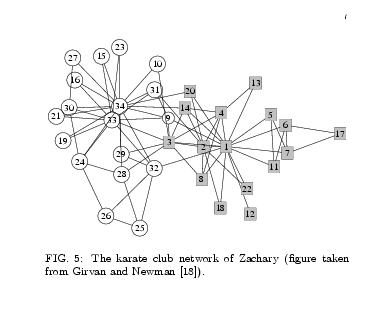
\includegraphics[scale=0.3, angle=-90]{graphe_karate.pdf} \\
\end{tabular}

\end{frame}

\begin{frame}
\frametitle{Questions induced by the network representation of the
data: the focus is on topological questions(2)}
\begin{tabular}{p{6cm}p{5cm}}

\vspace{0cm} \hspace{0cm}{\small  Are there clusters composed of
highly connected nodes?
    something like connected components in a weak sense. \begin{itemize}
        \item the rare edges between the clusters are the most important ones for the network's connectivity.
        \item If a node A, with unknown properties, is in the same cluster that a
        well known node B, then we are tempted to attribute B's properties to
        A.
    \end{itemize}}
    &
     \vspace{0cm} \hspace{-2.5cm}
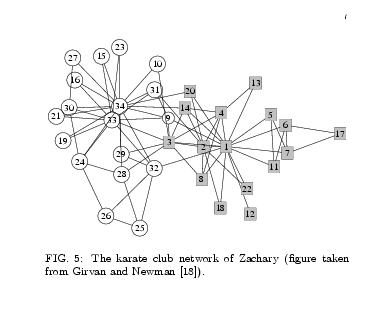
\includegraphics[scale=0.3, angle=-90]{graphe_karate.pdf} \\
\end{tabular}

\end{frame}



\begin{frame}
\frametitle{Questions induced by the network representation of the
data: the focus is on topological questions (3)}

\begin{tabular}{p{6cm}p{5cm}}
\vspace{0cm} \hspace{0cm}{\small
    \begin{itemize}
    \item How many hubs ? they are the most important nodes
    in the network. If they are suppressed, the network's
    connectivity is highly decreased.
    \item More generally, we are tempted to count some particular
    motifs (hub, triangle, square...). Some of them may be highly
    frequent so that we can characterize a network by its most frequent
    motifs.
    \item Resilience of the network's connectivity to edge suppression.
\end{itemize}}
    &
     \vspace{0cm} \hspace{-2.5cm}
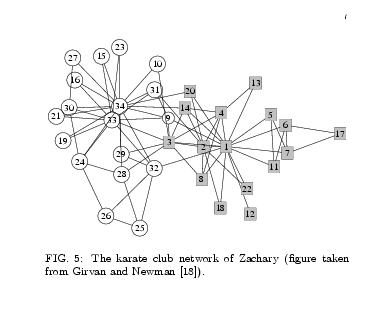
\includegraphics[scale=0.3, angle=-90]{graphe_karate.pdf} \\
\end{tabular}

\end{frame}

\begin{frame}
\frametitle{Data and Questions for which the network
representation seems less useful}

    \begin{itemize}
    \item Weighted networks with more than 10 nodes
    \item  Supervised classification of nodes (prediction of the function of
 proteins...)
    \item Supervised classification of edges.
\end{itemize}


\end{frame}

\section{Some basic definitions and properties about networks}

\begin{frame}
\frametitle{Some basic definitions and properties about networks}
\end{frame}

\begin{frame}
\frametitle{Basic definitions}
\begin{tabular}{p{6cm}p{5cm}}
\vspace{0cm} \hspace{0cm}
  \begin{itemize}
    \item A graph is $G=(V,E)$ where $V$ is a set of vertices (or
    nodes) and $E$ is a set of values corresponding to each couple of vertices
    $V$.
    \item If the values of $E$ are real, $G$ is valued and is
    called a {\it weighted or valued graph}.
    \item If the values of $E$ are in $(0,1)$, $G$ is called
    {\it a direct graph}.
    \item If the values of $E$ are in $(0,1)$  and $e_{ij}=e_{ji}  \forall (i,j) \in V$, $G$ is
    called {\it undirected graph}.
\end{itemize}
    &
     \vspace{0cm} \hspace{0cm}
\includegraphics[scale=0.2, angle=0]{barabasi1.pdf} \\
\end{tabular}

\end{frame}


\begin{frame}
\frametitle{Basic definitions for undirected graphs}

\includegraphics[scale=0.5, angle=0]{ClipBoard.png}\\
\begin{tabular}{p{7cm}p{5cm}}

   \vspace{0cm} \hspace{-1cm}

     \begin{description}
       \item[Adjacency matrix] $X$  with $X_{ij}=1$ if node $i$
       is connected to node $j$ and else $X_{ij}=0$.
       \item[Degree of node $i$] $K_i=\sum_jX_{ij}$
       \item[Distance between $i$ and $j$] length of the shortest
       path between $i$ and $j$
       \item[clique] a clique  is a set of vertices, such that for
       every two vertices, there exists an edge connecting them.
   \end{description}
    &
   \vspace{-1.5cm}
  \begin{tabular}{c}
\begin{equation*}
    X=\left(
    \begin{array}{ccccc}
  0 & 1 & 1 & 0 & 0 \\
  1 & 0 & 1 & 1 & 0 \\
  1 & 1 & 0 & 0 & 0 \\
  0 & 1 & 0 & 0 & 1 \\
  0 & 0 & 0 & 1 & 0
   \end{array}
    \right)
\end{equation*} \\

     \\
     \\
     $K_1=2$, $K_2=3$, $K_3=2$,\\
     $K_4=2$, $K_5=1$
     \\
     \\
     $D(3,5)=3$ \\
     \\
     (1,2,3) is a clique\\
   \end{tabular} \\
\end{tabular}

\end{frame}



\section{Characterization of a network by the counts of some topological motifs}

\begin{frame}
\frametitle{Characterization of a network by the counts of some
topological motifs}
\end{frame}


\begin{frame}
\frametitle{Topological motifs} {\small
\begin{tabular}{|c|c|}
  \hline
  z(x) & description \\
  \hline
  $k$-degree & number of nodes with degree $k$ \\
  Triangle & number of triangles \\
  V & number of V \\
  C & 3(number of triangles)/ number of V \\
  Squares & number of squares \\
  $k$-star & number of nodes with $k$ edges with unconnected endpoints \\
  geodesic & length of the longest distance between two nodes \\
  edge count & number of edges \\
  ... & ... \\
  \hline
\end{tabular}
}
\end{frame}

\begin{frame}
\frametitle{Empirical distribution of the degrees of a chemical
reaction network {\tiny V. Lacroix, M-F. Sagot }} \vspace{-1cm}
\includegraphics[height=12cm, angle=-90] {dist_emp_degr_coli.pdf}
\end{frame}


\begin{frame}
\frametitle{Degrees pdf "scale free", popular in the physicist
community 5 years ago}
$$
P(K=k)=c(\rho)k^{-(\rho)}
$$
with $k \in N$, $k>k_0$, $\rho>1$ et
$$c(\rho)=\left[\sum_{k>k_0} k^{-(\rho)}\right].$$
Scale free $\leftrightarrow$ $\frac{P(K=\alpha
k)}{P(K=k)}=\frac{(\alpha
k)^{-(\rho)}}{k^{-(\rho)}}=\alpha^{-\rho}$ do not depend on $k$.\\
$$log(P(K=k))=log(c(\rho))-\rho logk$$
log-log plot $y-axis$: $log(\widehat{P}(K=k))$, $x-axis$: $logk$.
\end{frame}


\begin{frame}
\frametitle{Log-Log-Plot for the reaction network} \vspace{-1cm}
\includegraphics[height=12cm, angle=-90 ] {loglogplot.pdf}
\end{frame}


\begin{frame}
\frametitle{Scale-free, an ubiquitous pdf ? {\tiny Newman 2002}}
\vspace{-3cm} \hspace{-3cm}
\includegraphics[height=20cm, angle=0 ] {newmanloglog.pdf}
\end{frame}

\begin{frame}
\frametitle{Building the network by preferential attachment lead
to scale-free networks {\tiny Barabasi 2002}}
\begin{tabular}{p{7cm}p{3cm}}
\vspace{-0.3cm}
\includegraphics[scale=0.3] {Barabasi7.png} &
\vspace{1cm} Two basic mechanisms
\begin{itemize}
    \item Growth
    \item Preferential attachment to nodes with high degree.
\end{itemize}
\\
\end{tabular}
\end{frame}

\begin{frame}
\frametitle{Five years later...}
\begin{itemize}
    \item Other pdf fit the empirical distribution of
    the degrees better than the scale-free pdf,
    \item The degree distribution is a poor information on the
    network topology.
    \item Samples of  scale-free networks are not scale-free.
\end{itemize}
\end{frame}

%\begin{frame}
%\frametitle{Log-Log-Plot(2)} \vspace{-1cm}
%\includegraphics[height=12cm, angle=-90 ] {loglogplot.pdf}
%\end{frame}
%
%\begin{frame}
%\frametitle{Fit of theoretical distributions for the degrees}
%\vspace{-1cm}
%\includegraphics[height=12cm, angle=-90 ] {dist_degr_coli.pdf}
%\end{frame}


\begin{frame}
\frametitle{Triangle Coefficient (C)} \vspace{-6cm}
\includegraphics[height=7cm, width=7cm] {V.pdf}
$$
C=P(T/V)
$$
 $T$ is a triangle and $V$ is a "V". \\
[0.5cm] The degree distribution and the C are partial and quite
poor statistics for characterizing the network.
\end{frame}


\begin{frame}
\frametitle{Characterization of a network by its degrees and C
{\tiny  Barabasi et al}} \vspace{-1.5cm}
\includegraphics[height=10cm, width=10cm] {Barabasi4.pdf}
\end{frame}

\begin{frame}
\frametitle{ Recent developments of Exponential Random Graph
Models, ERG or $p^*$ models, {\tiny  from Robins, Snijders,
Handcock, Pattison 2007}}
$$P(X=x)=\frac{e^{\theta'z(x)}}{C(\theta)}$$
\begin{itemize}
    \item $\theta$ is a $p$-vector of
parameters
    \item $z(x)$ is a $p$-vector
of motifs statistics.
\end{itemize}

A network is characterized by $\widehat{\theta}$. This allows
comparison between networks, by comparing their parameters
estimates $\widehat{\theta}$. \\ Saul et al. Bioinformatics 2007,
compared 43 metabolic networks using ERG models.
\end{frame}



\begin{frame}
\frametitle{Exceptional motifs in a network}
\includegraphics[height=5cm, width=11.5cm] {Motif1.png}
\end{frame}

\begin{frame}
\frametitle{Exceptionally frequent motifs in a network} 209 motifs
"bi-fan"  in a directed gene regulation network of {\it E. Coli}
\vspace{-0.5cm}
\includegraphics[height=7cm, width=7cm] {Barabasi5.pdf}
\end{frame}


\begin{frame}
\frametitle{Is the count exceptional ? {\tiny Shen-Orr 2002}}
\includegraphics[height=5cm, width=11cm] {Motif2.png}


The results depend on the reference model, see Picard 2007.
\end{frame}

\section{Nodes clustering}

\begin{frame}
\frametitle{Nodes clustering}
\end{frame}

\begin{frame}
\frametitle{Clustering of nodes}

\includegraphics[scale=0.5, angle=0]{communities.png} \\
Santa Fe Institute collaboration network: the nodes of the network
represent scientists from the Santa Fe Institute and an edge is
drawn between two nodes if the corresponding scientists have
coauthored at least one publication during the calendar year 1999
or 2000.

\end{frame}


\begin{frame}
\frametitle{Clustering methods}
\begin{description}
    \item[Hierarchical clustering] a well-known set of algorithms
    for a similarity matrix, many criteria proposed
    \item[Spectral clustering]: k-means on the space associated to the $q$-lowest eigenvalues of the Laplacian
    of the network, $D-X$, with $D=diag(sum(X))$ {\tiny tutorial from U. Von Luxburg, Stat Comput,
    2007}.
    \item[Markov Clustering Algorithm] MCL simulates a flow on the
    graph by calculating successive powers of $X$. At each
    iteration an inflation step is applied to enhance the contrast
    between regions of strong or weak flow in the graph. The
    process converges towards a partition of the graph, with a set
    of high flow regions separated by boundaries with no flow,
    {\tiny package from Von Dongen}
    \item[Edge-betweenness clustering] Divisive method using the
edge betweenness EB, (for an edge) : the number of shortest paths
that pass through the edge. The edge with the highest EB is
removed, {\tiny  Girvan \& Newman}
\end{description}
\end{frame}


\begin{frame}
\frametitle{Statistical models for clustering}
\begin{description}
        \item [Discrete latent variable,  $Z$]
        $$P(X_{ij}=1/Z_i=q,Z_j=l)=\pi_{ql},$$ {\tiny packages BLOCKS 1.6 (Snijders et al.) and  ERMG
        05, (Robin et al.)}, the clusters obtained are not necessarily
        highly connected within clusters and poorly connected
        between clusters.
        \item [Continuous latent variables, $Z$]  $$\frac{P(X_{ij}=1/Z_i=z_i,Z_j=z_j)}{P(X_{ij}=0/Z_i=z_i,Z_j=z_j)}=e^{\beta(z_i-z_j)}$$
         where $Z$ has a multivariate gaussian
        mixture pdf, {\tiny package latentnet, Handcock et al.}
    \end{description}
    Estimation methods: MCMC or variational ML.

\end{frame}

\begin{frame}
\frametitle{Clusters in the model using a discrete latent
variable}
  \begin{table}[h]
    \begin{center}
      \begin{tabular}{lccc}
        \hline
        Description & Graph & $Q$ & $\pibf$ \\
        \hline
        \begin{tabular}{p{2cm}} Erdos \end{tabular}
        & \begin{tabular}{c}
          \includegraphics[height=1.7cm,width=2.3cm]{FigNetworks-Erdos.pdf}
        \end{tabular}
        & 1
        &  $p$ \\
        \hline
        \begin{tabular}{p{2cm}} Star \end{tabular}
        &
        \begin{tabular}{c}
          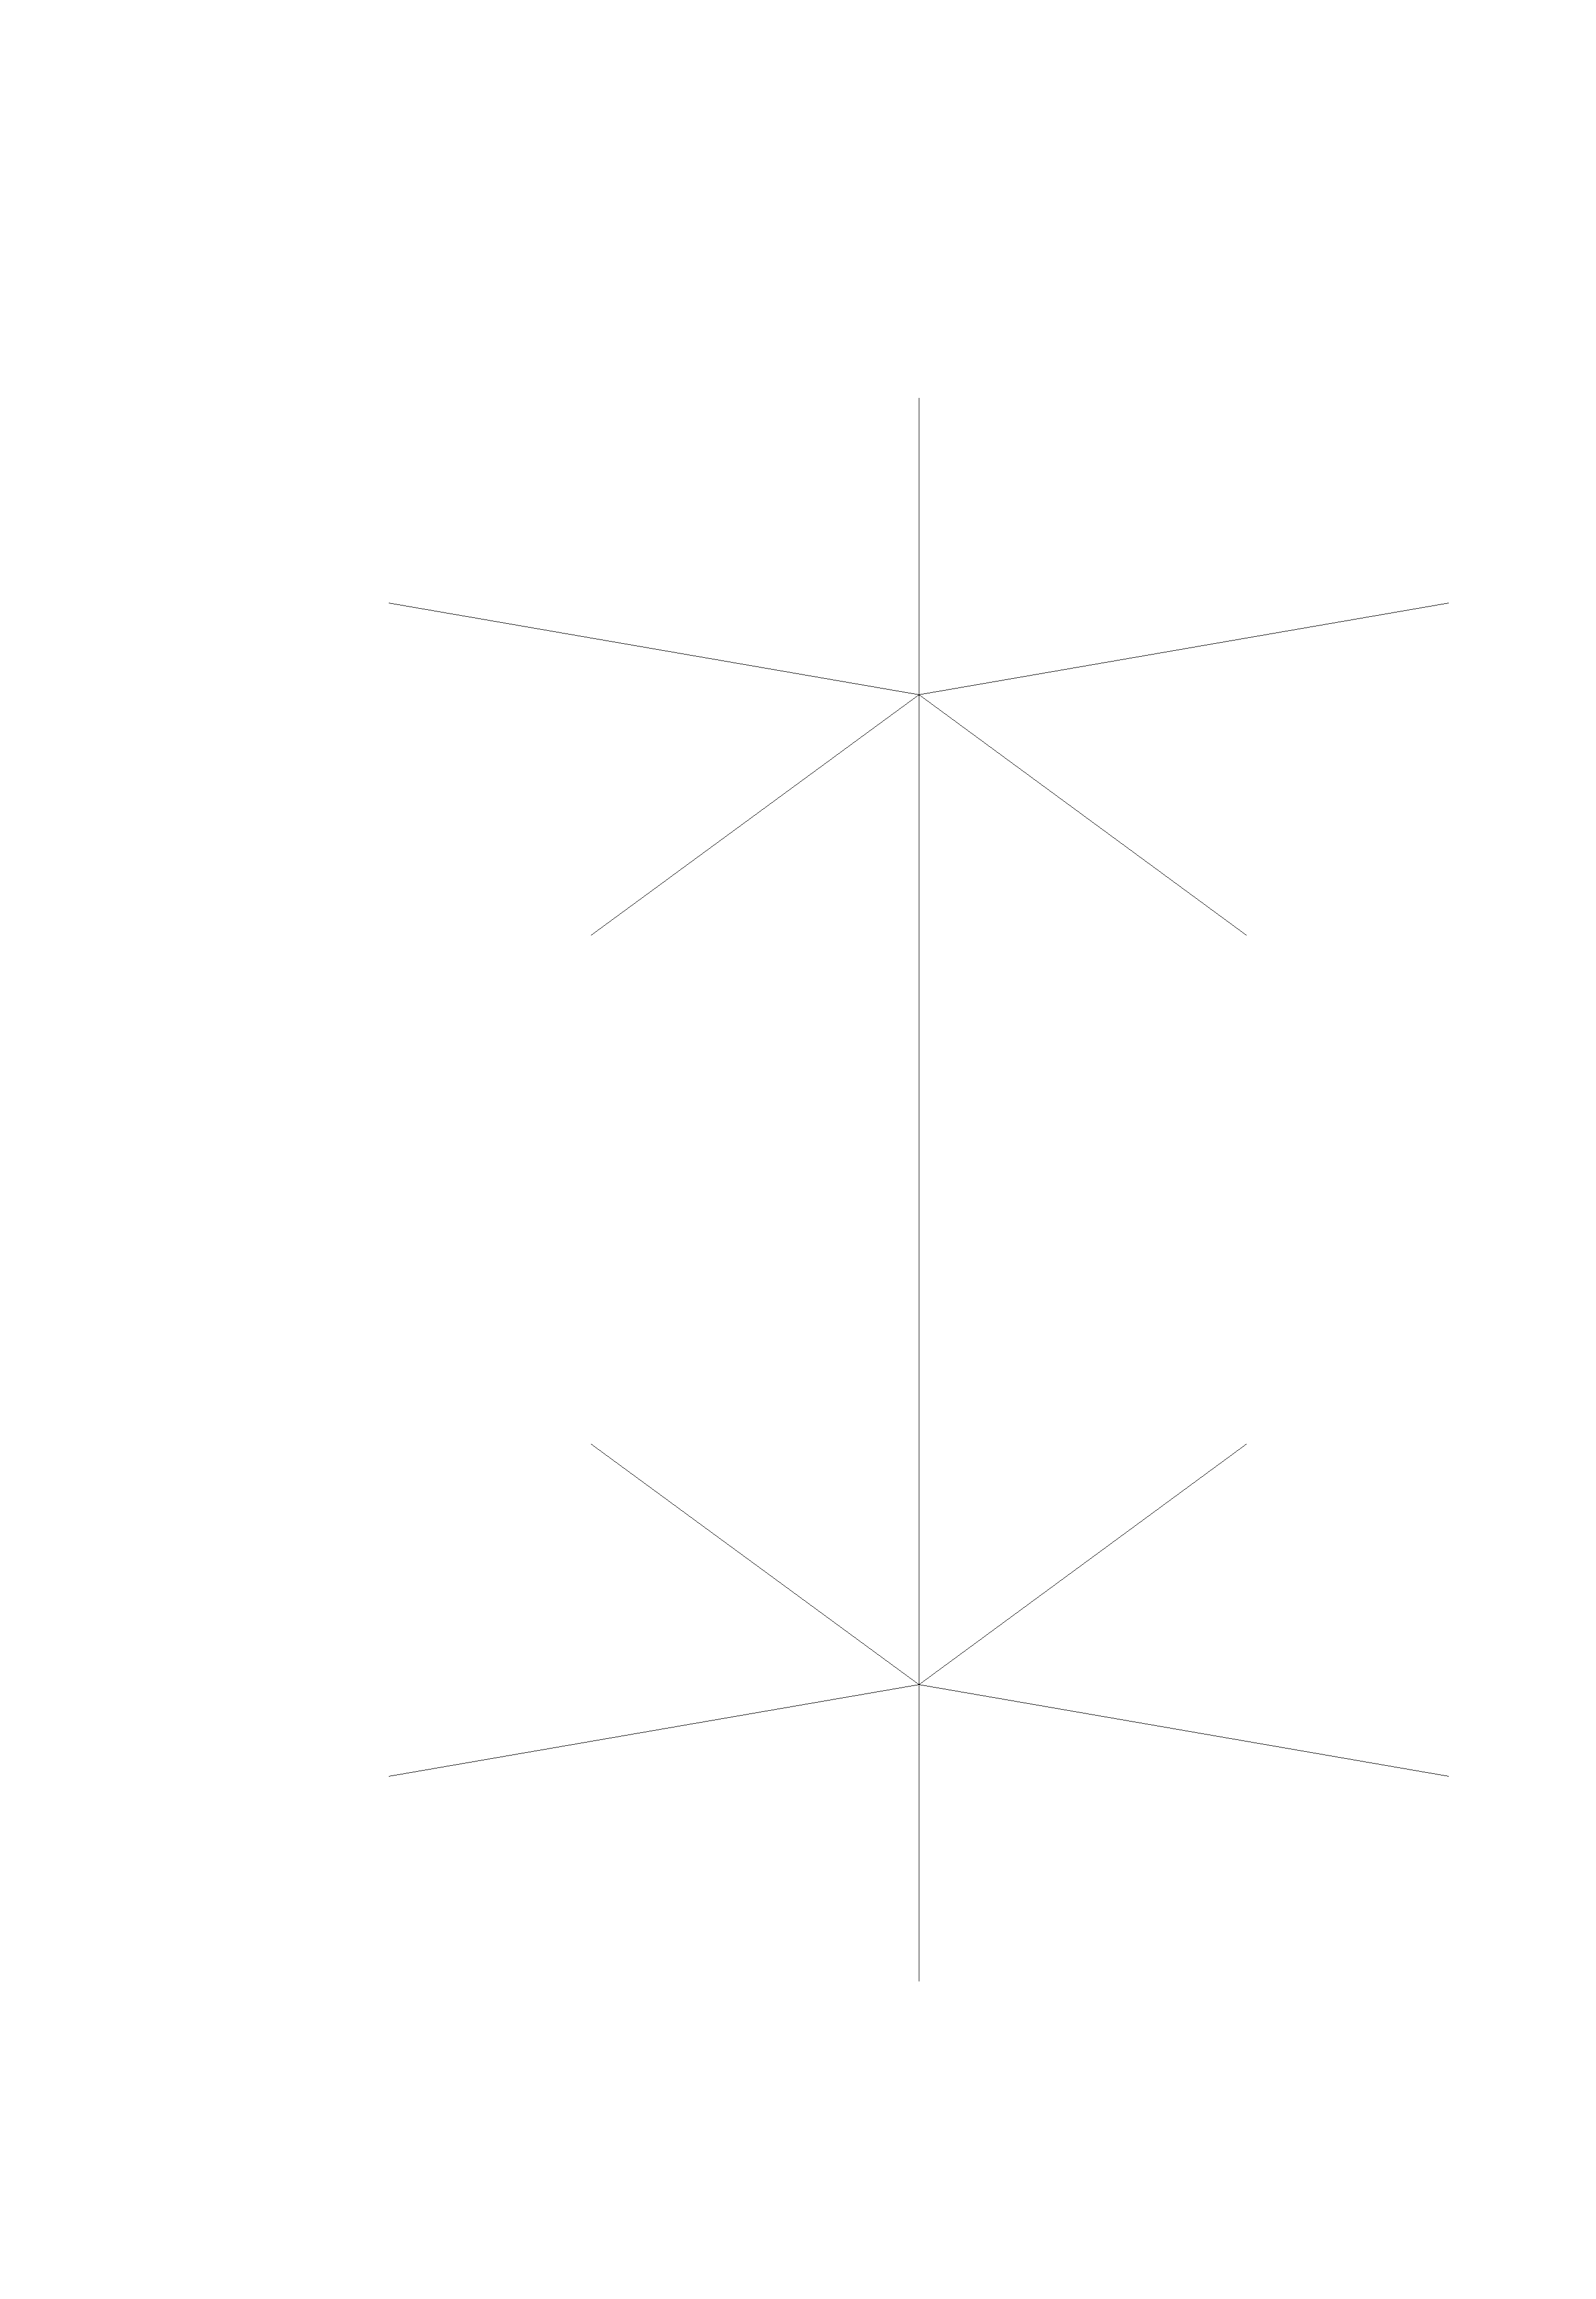
\includegraphics[height=1.7cm,width=2.3cm]{FigNetworks-Star.pdf}
        \end{tabular}
        & 4
        & $\left( \begin{array}{cccc} 0&1&0&0\\ 1&0&1&0\\0&1&0&1\\0&0&1&0\\
          \end{array} \right)$
         \\
        \hline \begin{tabular}{p{2cm}}  cluster in usual sense
        \end{tabular}

        & \begin{tabular}{c}
          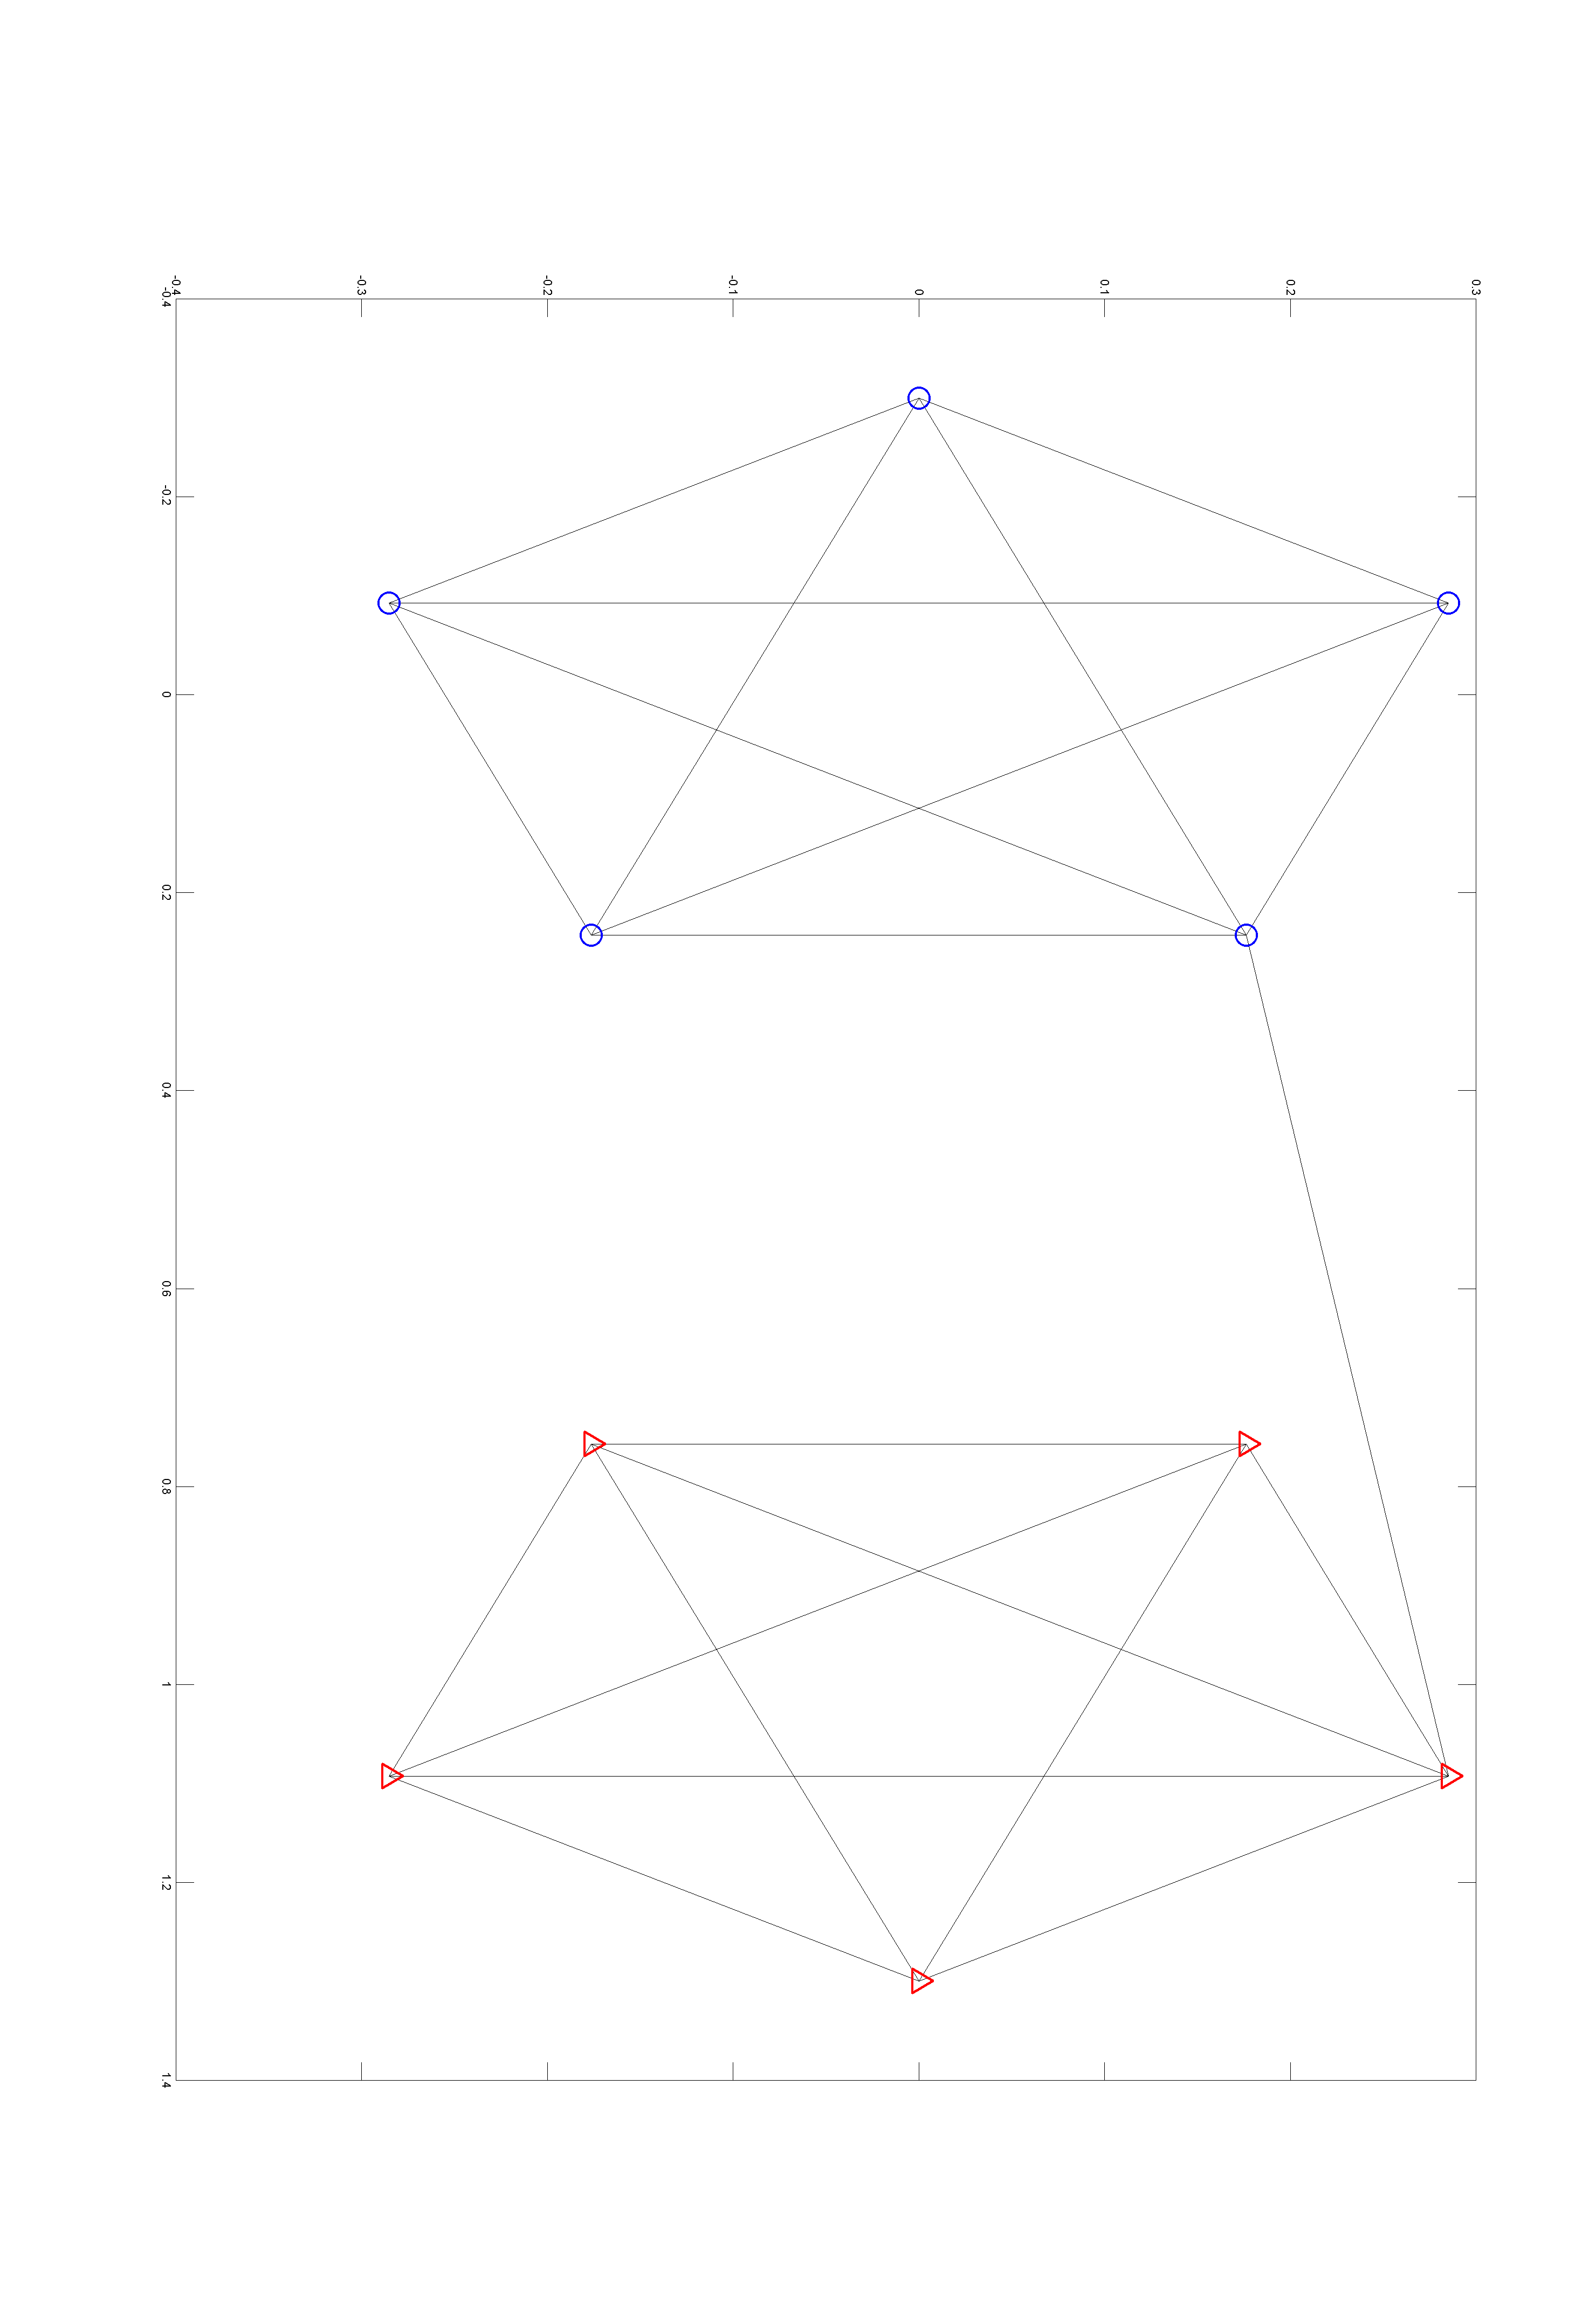
\includegraphics[height=1.7cm,width=2.3cm]{FigNetworks-Clusters.pdf}
        \end{tabular}
        & 2
        & $\left(\begin{array}{cc} 1&\varepsilon\\ \varepsilon&1\\
          \end{array} \right)$ \\
        \hline
      \end{tabular}
    \end{center}
  \end{table}

\end{frame}

\begin{frame}
\frametitle{Continuous latent variables and Principal Coordinate
Strategy}

\begin{tabular}{ccc}
  Relational data & PCO  & Usual data structure \\

\begin{tabular}{|c|c|c|}
    \hline
    item1 & item2 & $R$ \\
    \hline
    1 & 2 & $r_{12}$  \\
    1 & 3 & $r_{13}$ \\
    . & . & .  \\
    $n-1$ & $n$ & $r_{n-1,n}$  \\
    \hline
  \end{tabular}
  & $\rightarrow$
  &
  \begin{tabular}{|c|c|c|c|c|}
    \hline
    item &$Z_1$ & ... & ... & $Z_k$\\
    \hline
    1 & $Z_{11}$ & ... & ... & $Z_{1k}$ \\
    2 & $Z_{21}$ & ... & ... & $Z_{2p}$ \\
    . & . & . & . & . \\
    $n$ & $Z_{n1}$ & ... & ... & $Z_{nk}$ \\
    \hline
  \end{tabular}
  \\
\end{tabular}
\\[1cm]

Then, it is easy to merge the individual data set $X$ and the
latent data set $Z$ because they have the same structure.\\ This
strategy, combined with kernel methods, has been used by Vert and
Yamanishi for system biology.
\end{frame}

\section{Class prediction for nodes}
\begin{frame}
\frametitle{Class prediction for nodes}
\end{frame}

\begin{frame}
\frametitle{Prediction of the function of a protein}
\includegraphics[height=7cm, width=12cm] {PredictionPPI1.png}
\end{frame}


\begin{frame}
\frametitle{Function prediction of a protein: basic idea}
\includegraphics[height=7cm] {PredictionPPI.png}
\end{frame}


\begin{frame}
\frametitle{Direct prediction versus prediction after clustering}
\includegraphics[height=7cm, width=12cm] {PredictionPPI2.png}
\end{frame}

\begin{frame}
\frametitle{Direct prediction using Markov Random Fields}
 $$   P[L(i)=1/L(V(i))]=f[\log(\pi/(1-\pi))+\beta N(i,1)+\alpha
    [N(i,1)-N(i,0)]-N(i,0)]$$
with \\
\begin{itemize}
    \item $L(i)$ is the label of node $i$,
    \item $N(i,1)$
(resp. N(i,0)) is the number of neighbors of $i$ with label 1
(resp. 0),
    \item $\pi$ is the marginal probability of labels 1
    \item $V(i)$
is the set of neighbors of $i$,
    \item $f(t)=1/(1+exp(-t))$
\end{itemize}
\end{frame}

\section{Statistical models for networks}

\begin{frame}
\frametitle{Statistical models for networks}
\end{frame}

\begin{frame}
\frametitle{ Basic model for random networks,
"Erd\"{o}s-R\'{e}nyi"}
 $$ \forall (i,j), P(X_{ij}=1)=p.$$
 $X_{i,j}$ are iid Bernoulli($p$).\\[0.5cm]
Historically and theoretically very important model, but too
simple in practice.\\ [0.5cm] Does not fit real data in any
domain.
\end{frame}

\begin{frame}
\frametitle{Statistical models for networks} More probabilistic
models for networks are necessary to:\begin{enumerate}
    \item summarize the information contained in one network and
    compare networks
    \item have a reference model to say if a particular motif is
    exceptional
    \item predict the label of a node
    \item predict the value of an edge
    \item create artificial networks by simulation
\end{enumerate}
\end{frame}

\begin{frame}
\frametitle{Conclusions}
\end{frame}

\begin{frame}
\frametitle{Complex networks = a speculative bubble or a true new
scientific topic for statisticians ?}
\begin{itemize}
    \item High level of "buzz" has interested many researchers on
    this topic $\rightarrow$ new models and new results
    \item \alert {In many domains (system biology, social sciences...) new data sets contain both individual and relational
    informations}. \\Example of the prediction of the function of proteins \begin{enumerate}
        \item PPI network (relational data)
        \item Blast score of AA or cDNA sequence (individual and
        relational data)
        \item Gene Ontology (individual data)
        \item Microarray expression data (individual data)
    \end{enumerate}
    \item The network plot is sometimes nice and fruitful and
    sometimes unnecessary and misleading.
\end{itemize}


\end{frame}

\begin{frame}
\frametitle {Future challenges} {\small
\begin{itemize}
\item Weighted networks ($r_{ij}\in \mathbb{R}$)
    \item  Multivariate relational data \\[0.5cm]
    \hspace{-1cm}
    \begin{tabular}{cc}
  Informations on items & Informations on relations between items \\
  \begin{tabular}{|c|c|c|c|c|}
    \hline
    item &$X_1$ & ... & ... & $X_p$\\
    \hline
    1 & $x_{11}$ & ... & ... & $x_{1p}$ \\
    2 & $x_{21}$ & ... & ... & $x_{2p}$ \\
    . & . & . & . & . \\
    $n$ & $x_{n1}$ & ... & ... & $x_{np}$ \\
    \hline
  \end{tabular}
     &
     \alert{
\begin{tabular}{|c|c|c|}
    \hline
    item1 & item2 & $R$ \\
    \hline
    1 & 2 & $r_{12}^{(1)}$, $r_{12}^{(2)}$ ,...$r_{12}^{(q)}$   \\
    1 & 3 &  $r_{13}^{(1)}$, $r_{13}^{(2)}$ ,...$r_{13}^{(q)}$  \\
    . & . & .  \\
    $n-1$ & $n$ & $r_{n-1,n}^{(1)}$, ...$r_{n-1,n}^{(q)}$  \\
    \hline
  \end{tabular}
  }
  \\
\end{tabular}
  \item \\[1cm] Individual and relational data indexed by the time $t$.

\end{itemize}
}
\end{frame}

\begin{frame}
\frametitle{Some References}
\end{frame}

\begin{frame}
\frametitle{References in the domain of System Biology}
    \begin{itemize}
\item  Barabasi A-L., Oltvai Z. {\it Network biology:
understanding the cell's functional organization}, Nature reviews,
Genetics, 5,fev 2004. \item  Palla G. Der�nyi I. Farkas I. and
Vicsek I. {\it Uncovering the overlapping community structure of
complex networks in nature and society}, Nature 435, 814-818 (9
June 2005)
 \item
Sharan R., Ulitsky I. and Shamir R.  {\it Network-based prediction
of protein function}, Molecular Systems Biology, 3, Article 88,
2007 \item AIttokallio T. and Schwikowski  B.  {\it Graph-based
methods for analysing networks in cell biology}, Briefings in
bioinformatics, 7,3, pp 243-255, 2006.
\item Y. Yamanishi, J.-P.
Vert  and M. Kanehisa  {\it Protein network inference from
multiple genomic data: a supervised approach}, Bioinformatics 20,
2004.
    \end{itemize}
\end{frame}

\begin{frame}
\frametitle{References in Ecology}
    \begin{itemize}
        \item  Lewinsohn T.M. and Prado P.I. {\it Structure in plant-animal interaction assemblages}, Oikos,113,1, 2006.
    \end{itemize}
\end{frame}

\begin{frame}
   \frametitle{References in the physicist community}
    \begin{itemize}
        \item A. Barabasi, Depart. of Physics, University of Notre
        Dame, $http://www.nd.edu/~alb/$
        \item P.E. Newman, Depart. of Physics, University of Michigan,
        $http://www-personal.umich.edu/~mejn/$
    \end{itemize}
\end{frame}


\begin{frame}
\frametitle{Exceptional motifs counts in networks}
    \begin{itemize}
        \item {\it An extended transcriptional regulatory network of E. Coli and analysis of its
         hierarchical structure and network motifs},
        NAR, 2004,32,22, 6643-6649
        \item Matias C., Schbath S., Birmele E., Daudin J.J., Robin S.,
        {\it Networks motifs mean and variance for the count},
        Revstat,4,1,2006.
        \item {\it Motifs, themes and thematic maps of an integrated
        Saccharomyces C. interaction network}, Journal of Biology, june 2005.
        \item  R. Jiang,Z.Tu, T. Chen and F. Sun {\it Network motif identification in stochastic
        networks} PNAS, juin 2006
        \item  Picard F., Daudin J.J., Schbath S. and Robin S. {\it Assessing the exceptionality of network motifs}
        SSB Research Report No. 1, November 2006.
    \end{itemize}
\end{frame}

\begin{frame}
\frametitle{Models for graphs}
    \begin{itemize}
\item Barabasi,  $http://www.nd.edu/~alb/$
\item M. Middendorf, E.
Ziv and C.H. Wiggins {\it Inferring network mechanisms: the
Drosophilia melanogaster protein interaction network}, PNAS, mars
2005
\item G. Robbins, T. Snijders, P. Wang, M. Handcock, P. Pattison
{\it Recent developments in exponential random graph ($p^*$)
models for social networks}, Social networks 29(2007), 192-215.
 \item M.S. Handcock and A.
E.Raftery and J. M. Tantrum {\it Model-based clustering for social
networks}, JRSSA, mars 2007
\item ERMG : Daudin J.J, Picard F.,
Robin S., {\it Mixture Model for Random Graphs: A Variational
Approach}, SSB Research Report No. 4, February 2007
\end{itemize}
\end{frame}

\begin{frame}
\frametitle{Clustering of nodes of networks}
    \begin{itemize}
     \item U. Von Luxburg, {\it A tutorial on spectral clustering}
  Statistics and Computing (2007), 17 395:416
        \item Brohee S. Van Helden, J. {\it Evaluation of clustering algorithms for protein-protein interaction
        networks}, BMC Bioinformatics, novembre 2006
\end{itemize}
\end{frame}

\begin{frame}
\frametitle{Thank you for your attention}
\end{frame}
\end{document}
